\iffalse
\documentclass[10pt,twocolumn]{article}
\usepackage{graphicx}
\usepackage[margin=0.5in]{geometry}
\usepackage[cmex10]{amsmath}
\usepackage{array}
\usepackage{booktabs}
\usepackage{mathtools}
\title{\textbf{Optimization}}
\author{Vemulapalli Bavya Sri}
\date{October 2022}


\providecommand{\norm}[1]{\lVert#1\rVert}
\providecommand{\abs}[1]{\vert#1\vert}
\let\vec\mathbf
\newcommand{\myvec}[1]{\ensuremath{\begin{pmatrix}#1\end{pmatrix}}}
\newcommand{\mydet}[1]{\ensuremath{\begin{vmatrix}#1\end{vmatrix}}}
\providecommand{\brak}[1]{\ensuremath{\left(#1\right)}}
\providecommand{\lbrak}[1]{\ensuremath{\left(#1\right.}}
\providecommand{\rbrak}[1]{\ensuremath{\left.#1\right)}}
\providecommand{\sbrak}[1]{\ensuremath{{}\left[#1\right]}}

\begin{document}

\maketitle
\paragraph{\textit{Problem Statement} -
\fi
It is given that at x=1, the function
$x^4-62x^2+ax+9$ attains its maximum value, on the interval [0,2]. Find the value of a. 
\\
\solution
\iffalse
\section{Solution}
\begin{flushleft}
Given function is,\\
\end{flushleft}
\begin{align}
\label{eqn:1}
    f(x)=x^4-62x^2+ax+9
\end{align}
\subsection{Calculation of Maxima using normal differentiation}
\begin{flushleft}
	\fi
Differentiating the given function,
\begin{align}
\nabla f(x) = 4x^3-124x+a
\end{align}
Since $f$ attains its maximum value on the interval [0,2] at $x=1$,
\begin{align}
\nabla f(1) =0
\implies a=120
\end{align}
\iffalse
\begin{flushleft}
\subsection{Calculation of Maxima using gradient ascent algorithm}
\end{flushleft}
\begin{flushleft}
Maxima of the above equation (1), can be calculated from the following expression,\\
To find,
\end{flushleft}
\begin{align}
\max_{x} f(x)
\end{align}  
\fi
Using gradient descent,
    \begin{align}
	    x_{n+1}&= x_n + \alpha \nabla f(x_n)
	    \\
	    &= x_n + \alpha \brak{4x_n^3-124x_n+120}
    \end{align}
    and choosing
\begin{align}
	x_0&=0.5,\alpha=0.001 \text{ and precision} = 0.00000001, 
	\\
	f_{max} &= 68,
        x_{max} = 1
\end{align}
	\begin{figure}[!ht]
		\centering
		\includegraphics[width=\columnwidth]{12/6/5/11/figs/b.png}
		\caption{}
		\label{fig:12/6/5/11}
  	\end{figure}
\iffalse
\end{flushleft} 
\center

\begin{flushleft}
\section{Construction}
\end{flushleft}

\begin{flushleft}
1. At first, the given function has been differentiated and it is solved by setting f'(x) equal to zero. By using x values, f(x) values are calculated.\\
\vspace{0.25cm}
2. Later, the given function f(x) is solved by gradient ascent algorithm to find maxima and the point at which f(x) is maximum.\\
\vspace{0.25cm}
3. Maxima and related points are, \\
\vspace{0.25cm}
\center
Maxima point, Max=(1 , 68) 
\end{flushleft}

\begin{figure}[h]
\includegraphics[scale=0.6]{b.png}
\caption{Graph}
\label{fig:Graph}
\end{figure}

\end{document}
\fi
